\section{Reproduced Results}
\label{sec:results}
\subsection{Profile Corpus and Failure Coverage}
All 21 stored labels match the rederived classifier, and the recorded content digest matches provenance. Table~\ref{tab:fixture} and Fig.~\ref{fig:fixture} show 12 target, eight minimum-useful, zero degraded, and one failed snapshot. The failure is the wearable profile's explicit unsupported offline coding request. The result follows directly from an offline state with $F_{c,w}=0$ in \eqref{eq:classifier}; it does not measure failed compilation or execution on a wearable.
\begin{table}[t]
\centering
\caption{Exhaustive counts in the 21 stored profile snapshots. No degraded or transitioning state is exercised.}
\label{tab:fixture}
\small
\begin{tabular}{lrrrr}
\toprule
Profile & Target & Degraded & Useful & Failed \\
\midrule
desk & 3 & 0 & 2 & 0 \\
mobile/docked & 3 & 0 & 2 & 0 \\
local/creation & 3 & 0 & 2 & 0 \\
wearable & 3 & 0 & 2 & 1 \\
\bottomrule
\end{tabular}
\end{table}


The three other profiles each have three target and two minimum-useful rows. The wearable has the same common five rows plus the unsupported request. This asymmetry prevents interpreting raw failure counts as fair comparative device reliability. The corpus deliberately probes a missing wearable capability while omitting analogous unsupported tasks for the other profiles.

\begin{figure*}[t]\centering
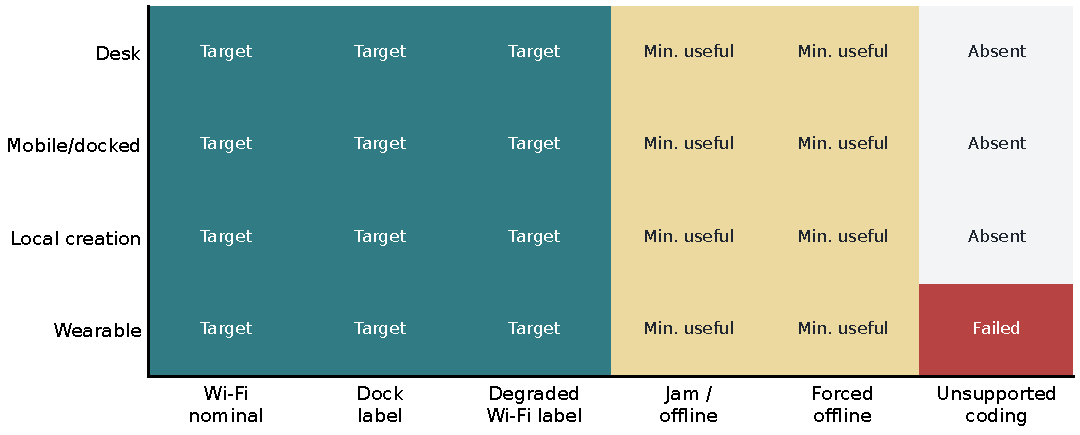
\includegraphics[width=0.91\textwidth]{figures/owner_fixture_matrix.pdf}
\caption{The 21 frozen snapshots. Absent cells are untested combinations. All four degraded-Wi-Fi labels retain connected state and therefore receive target. No snapshot exercises degraded or transitioning state.}\label{fig:fixture}
\end{figure*}

All four scenarios named degraded Wi-Fi receive target because their stored orchestrator state is connected. Hence the scenario label does not establish a degraded-service observation. The zero degraded count exposes a coverage gap in the fixture, even though the classifier has a degraded branch. The 20 Gary overlay rows contain no below-minimum-useful outcome because the context mapping selects declared supported workloads. This is a property of that mapping and workload selection, not evidence that all real disruptions preserve useful service.

The post hoc connected-only semantic comparator labels all nine offline rows failed. The benchmark instead identifies eight as minimum useful and one as failed. The eight reclassifications show precisely what the coverage declaration adds to a connectivity-only label. They do not quantify a policy improvement: no fallback action, application execution, or user benefit was measured in this comparison.

\subsection{Thirty-Seed Primary Outcomes}
Table~\ref{tab:primary} gives the reproduced overall outcomes. Task completion is 0.427257 with sample standard deviation 0.041610; useful occupancy is 0.591493 with standard deviation 0.040243. Their 95\% seed-level intervals are [0.411720,0.442795] and [0.576466,0.606520], respectively. Completion is bounded by useful occupancy at every class and step by \eqref{eq:task}; the lower completion mean reflects the conditional task-success gate.
\begin{table}[t]
\centering
\caption{Frozen seeded timeline outcomes; 95\% Student-$t$ intervals over 30 seed means.}
\label{tab:primary}
\small
\begin{tabular}{lrrl}
\toprule
Outcome & Mean & SD & 95\% CI \\
\midrule
Completion $C$ & 0.4273 & 0.0416 & [0.4117, 0.4428] \\
Useful time $\tau$ & 0.5915 & 0.0402 & [0.5765, 0.6065] \\
\bottomrule
\end{tabular}
\end{table}


\begin{figure}[t]\centering
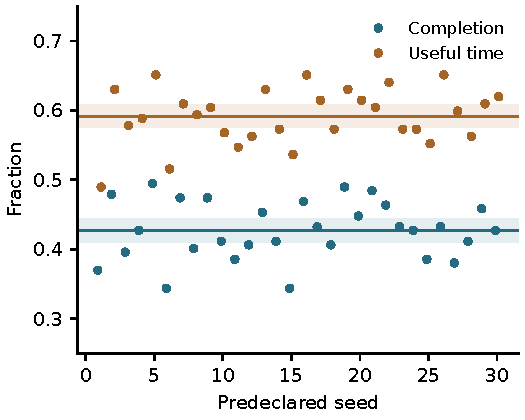
\includegraphics[width=\columnwidth]{figures/owner_seed_outcomes.pdf}
\caption{All 30 recorded seed means. Lines show means and shaded bands show their 95\% Student-$t$ intervals. These are intervals for generator means, not prediction bands for real deployments.}\label{fig:seeds}
\end{figure}

The observed overall completion range is approximately 0.344 to 0.495 and the useful-occupancy range 0.490 to 0.651 (Fig.~\ref{fig:seeds}). The intervals use all recorded seeds; none were removed based on outcome. Changing the seed set, step count, or prior values creates a different experiment and must be versioned separately.

\subsection{Class Priors and Analytic Interpretation}
The four timeline classes differ from the four profile categories. Table~\ref{tab:classes} therefore summarizes the stochastic classes independently. Wearable completion and useful occupancy are about 0.171 and 0.348; edge-node values are 0.628 and 0.786. The ordering is consistent with the authored probabilities and stress sensitivities.
\begin{table*}[t]
\centering
\caption{Timeline classes have synthetic resilience priors; intervals describe the generator, not measured hardware.}
\label{tab:classes}
\small
\begin{tabular}{lrlrl}
\toprule
Class & $C$ & 95\% CI & $\tau$ & 95\% CI \\
\midrule
wearable & 0.171 & [0.148, 0.193] & 0.348 & [0.320, 0.376] \\
smartphone & 0.392 & [0.365, 0.419] & 0.569 & [0.543, 0.594] \\
laptop & 0.519 & [0.491, 0.546] & 0.663 & [0.634, 0.692] \\
edge\_node & 0.628 & [0.596, 0.660] & 0.786 & [0.761, 0.811] \\
\bottomrule
\end{tabular}
\end{table*}


For $b_c=0.35h_c$, the unrounded model yields the post hoc expectations
\begin{align}
\mathbb E[\tau_c]&=a_c(1-b_c/2),\label{eq:exp_tau}\\
\mathbb E[C_c]&=a_cq_c\left[1-\frac{b_c+0.2}{2}+\frac{0.2b_c}{3}\right].\label{eq:exp_c}
\end{align}
These integrate \eqref{eq:useful} and \eqref{eq:task} over uniform stress. Expected completion values for wearable, smartphone, laptop, and edge node are 0.1721, 0.4203, 0.5243, and 0.6287; expected useful fractions are 0.3437, 0.5940, 0.6810, and 0.7722. Fig.~\ref{fig:classes} places these values beside the simulation estimates. The smartphone completion expectation lies just above its descriptive interval; the study has not performed a formal goodness-of-fit test or simultaneous-coverage assessment. The analytic calculation is a model interpretation, not an additional independent experiment.

\begin{figure}[t]\centering
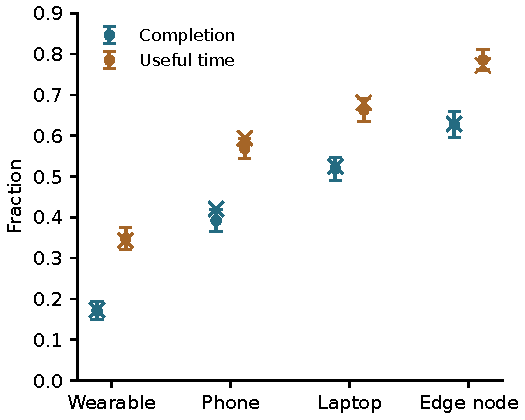
\includegraphics[width=\columnwidth]{figures/owner_class_outcomes.pdf}
\caption{Class means and descriptive 95\% intervals. Crosses mark post hoc analytic expectations. The class ordering reflects configured priors, with no calibrated hardware ranking implied.}\label{fig:classes}
\end{figure}

\subsection{Secondary Endpoint Audit}
The source defines reliability equal to useful occupancy. Outage fraction, QoE-violation fraction, and packet-loss proxy each equal its complement; throughput proxy is five times useful occupancy; compute-completion-time proxy is $T(1.2-0.4C)$. The identities hold up to reporting precision (Table~\ref{tab:metrics}). These fields are retained in machine-readable outputs for historical compatibility, but do not constitute independent validation of reliability, packet loss, quality of experience, throughput, or compute performance.

The field \texttt{recovery\_event\_count} increments when a failed step follows a non-outage step, including entry into an initial outage. It counts outage episodes entered, rather than successful recoveries. It is excluded from the aggregated secondary-key list. No recovery duration, restored-task fraction, or completed-recovery count is reported as an empirical result.

\begin{table}[t]\centering\caption{Metric meanings established by source inspection; historical field names are preserved in artifacts.}\label{tab:metrics}\small
\begin{tabular}{p{0.39\columnwidth}p{0.49\columnwidth}}\toprule
Reported field & Implemented definition and interpretation\\\midrule
Reliability & $\tau$; duplicate primary endpoint\\
Outage / QoE violation / packet-loss proxy & $1-\tau$; three duplicate complements\\
Throughput proxy & $5\tau$; arbitrary Mbps scaling\\
Compute completion proxy & $T(1.2-0.4C)$; synthetic transform\\
Recovery-event count & Number of outage entries; no completion test\\
Latency / jitter & Affine stress proxy / consecutive absolute differences\\
Energy proxy & Demand-weighted synthetic sum; no battery model\\\bottomrule
\end{tabular}\end{table}
